%Jasper is doing this

The safety subsystem determines whether it is safe to continue operation (unsafe conditions are when a human is detected too close to the operation area or the emergency stop is triggered). All operations should halt when unsafe conditions are detected.

\subsubsection{Safety Sensor Programming Languages}
Python/URScript

\subsubsection{Safety Sensor Software Dependencies}
URX Python library

\begin{figure}[h!]
	\centering
 	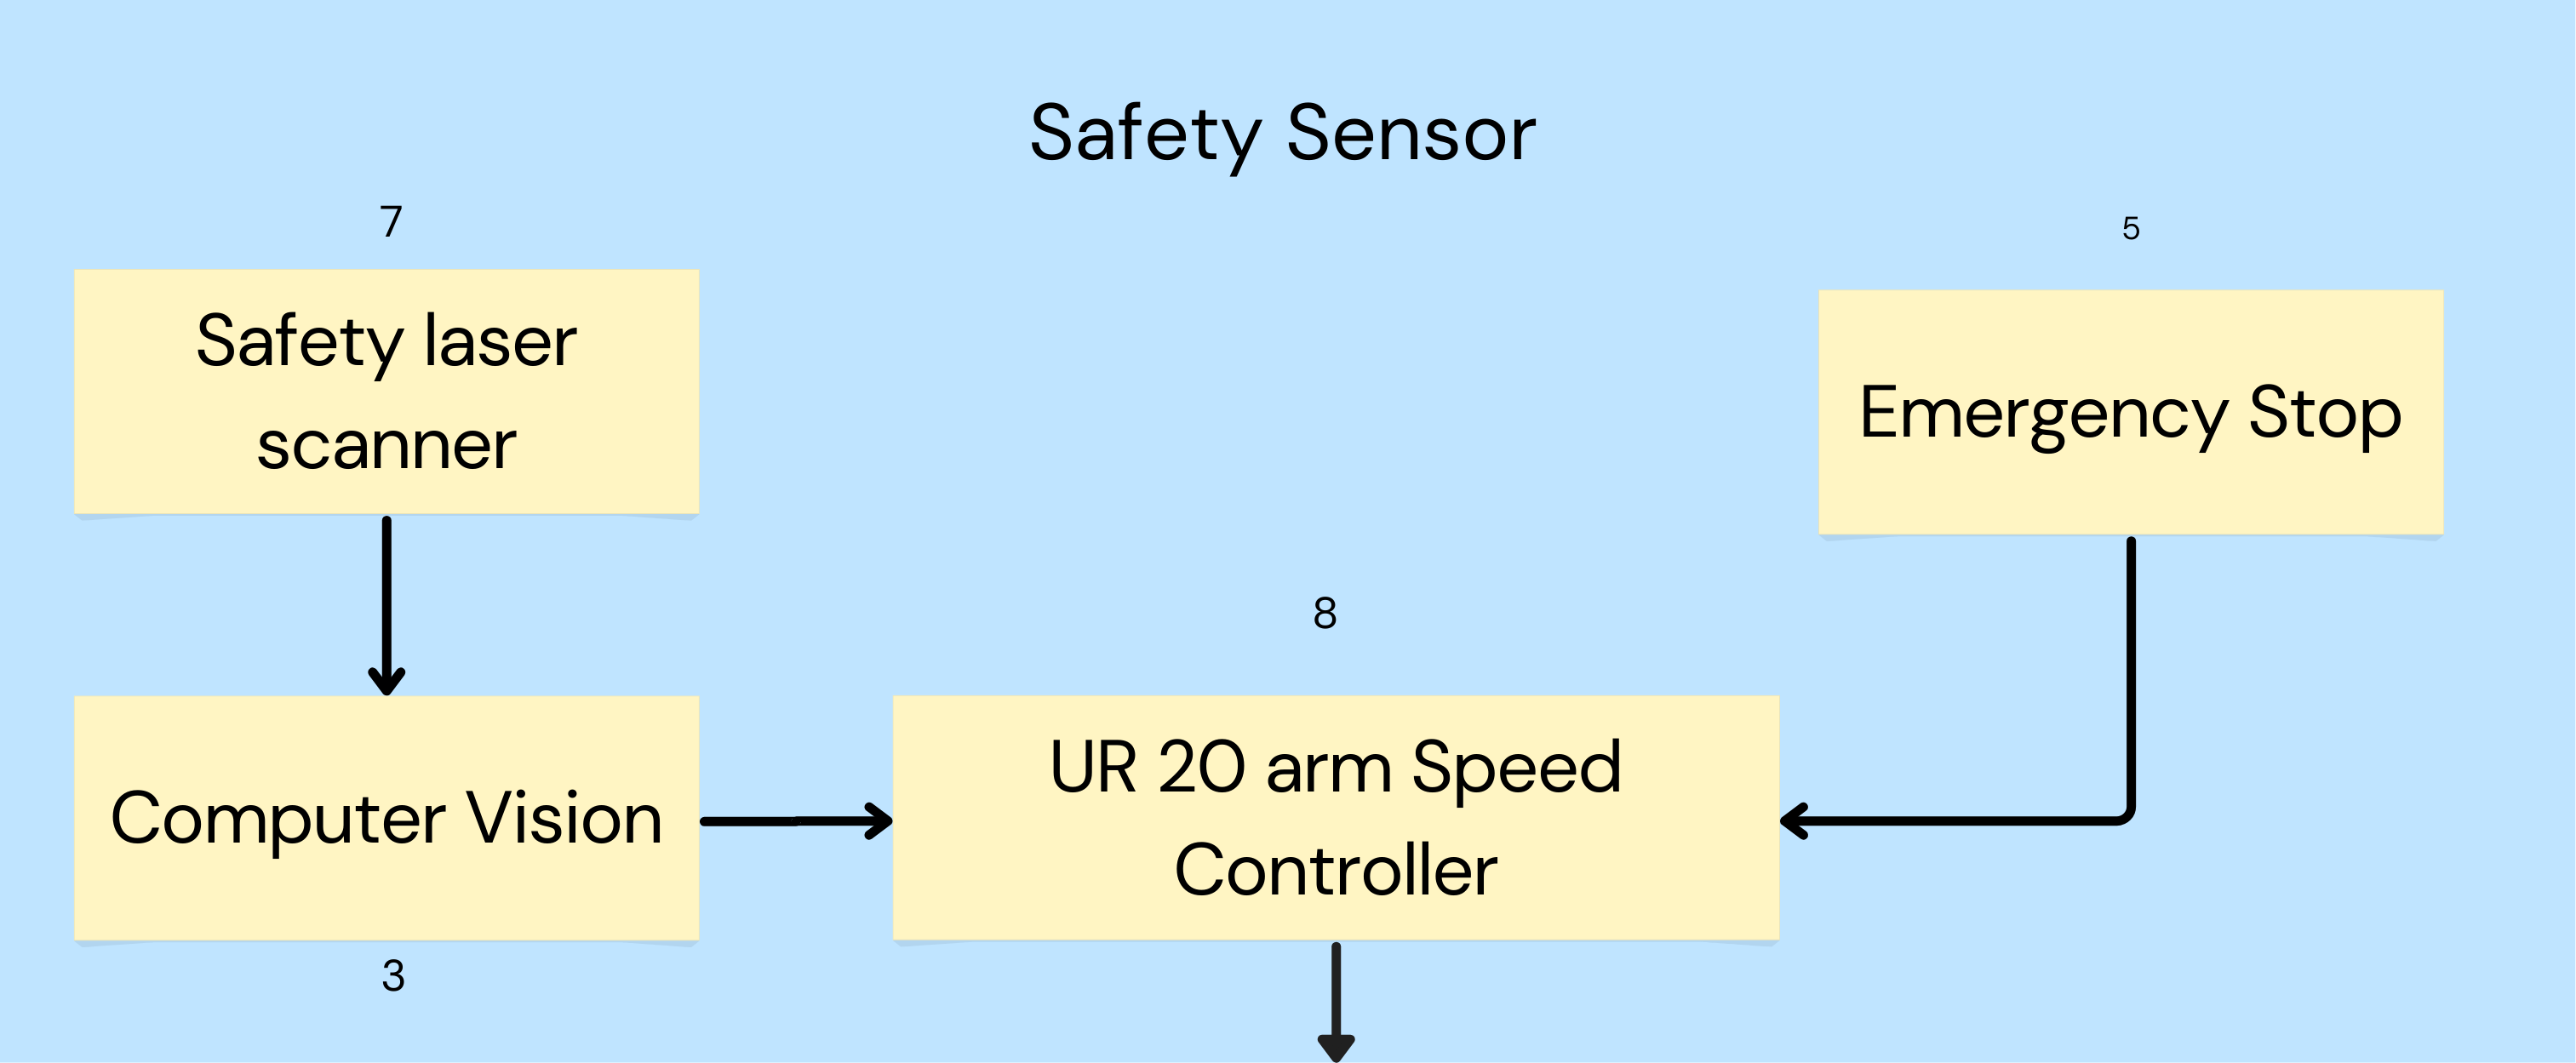
\includegraphics[width=0.60\textwidth]{images/safety.png}
 \caption{Safety sensor diagram}
\end{figure}

\subsection{Proximity Sensor Subsystem}
Detects the distance of a nearby person, if there is any person nearby.

\subsubsection{Proximity Sensor Hardware}
An IR proximity sensor mounted at the base of the robot arm, opposite the conveyor belt, detects the position and distance of any living creatures.


\subsection{Computer Vision Subsystem}
Detects if a person enters the operational area of the UR20 arm.

\subsubsection{Computer Vision Data Structures}
Receives data from the IR sensor. Details unknown due to recent change of plans.

\subsubsection{Computer Vision Data Processing}
We are not filled in on how detailed the IR sensor's data is, but if distance is not given then the number of beams 'blocked' will be use to estimate the apparent size of a nearby person.


\subsection{Speed Control Subsystem}
Determines the safest operational speed to perform at.

\subsubsection{Speed Control Data Structures}
Receives estimated distance of the nearest person from the Computer Vision subsystem.

\subsubsection{Speed Control Data Processing}
If a person is close but not within operational range, slow movement. If a person is within operational range, stop movement. Otherwise, operate at normal speed UNLESS the emergency stop is triggered, at which case ALL operation will be stopped, and if possible, manual repositioning mode will be enabled (where the arm can be moved by applying pressure).

\subsection{Emergency Stop Subsystem}
Triggers a complete stop of all operation.

\subsubsection{Proximity Sensor Hardware}
This is a physical button located on the 3PE Teach Pendant. 

\subsubsection{Proximity Sensor Data Structures}
This is integrated fully with the UR20's basic control system. A single signal will be sent to all modules that indicates whether the UR20 is controllable or in stop mode. In stop mode, no operation will be possible in any module.
